\documentclass[tikz,border=10pt]{standalone}
\usepackage{tikz}
\usetikzlibrary{calc}

\begin{document}
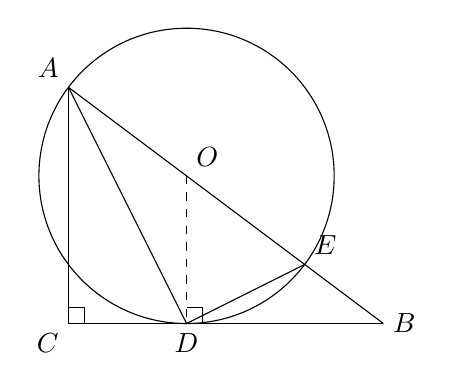
\begin{tikzpicture}
    \coordinate (C) at (0,0);
    \coordinate (A) at (0,3);
    \coordinate (B) at (4,0);
    \coordinate (O) at (1.5, 1.875);
    \coordinate (D) at (1.5, 0);
    \coordinate (E) at (3, 0.75);

    \draw (O) circle (1.875);
    \draw (A) -- (C);
    \draw (C) -- (B);
    \draw (A) -- (B);
    \draw (A) -- (D);
    \draw (D) -- (E);
    \draw[dashed] (O) -- (D);

    \draw (0, 0.2) -- (0.2, 0.2) -- (0.2, 0);
    \draw ($(D) + (0, 0.2)$) -- ($(D) + (0.2, 0.2)$) -- ($(D) + (0.2, 0)$);

    \node[above left] at (A) {$A$};
    \node[right] at (B) {$B$};
    \node[below left] at (C) {$C$};
    \node[below] at (D) {$D$};
    \node[above right] at (E) {$E$};
    \node[above right] at (O) {$O$};
\end{tikzpicture}
\end{document}
